%%
%% This is file `main.tex'
%%
%% ------------------------------------------------------------------------
%% Copyright (C) 2022 Q.Tang
%% 
%% Licensed under the Apache License, Version 2.0 (the "License");
%% you may not use this file except in compliance with the License.
%% You may obtain a copy of the License at
%% 
%%     http://www.apache.org/licenses/LICENSE-2.0
%% 
%% Unless required by applicable law or agreed to in writing, software
%% distributed under the License is distributed on an "AS IS" BASIS,
%% WITHOUT WARRANTIES OR CONDITIONS OF ANY KIND, either express or implied.
%% See the License for the specific language governing permissions and
%% limitations under the License.
%% ------------------------------------------------------------------------

\documentclass{bjtu-bachelor-thesis}
%========================================================================%
% 自定义内容
%========================================================================%

\author{XX}
\studentNumber{1730xxxx}
\advisor{XXX}
\school{软件学院}
\major{软件工程}
\title{设计(论文)题目}
\englishtitle{The Design and Implementation of \\ Thesis Template Based on \LaTeX}

%========================================================================%
% 前置部分
%========================================================================%

\begin{document}
\pagenumbering{roman}
\makecover % 封面
\makeAuthorization % 版权声明

\setcounter{page}{1}
\pagestyle{bjtufancy}

\begin{chineseabstract}	

\noindent\bjtusongti{\textbf{摘要:}}[鼠标左键单击选择该段落,输入替换之。内容为小四号宋体。] 中文摘要应将论文的内容要点简短明了地表达出来,约400字左右,字体为宋体小四号。内容应包括工作目的、研究方法、成果和结论。要突出本论文的创新点,语言力求精炼。为了便于文献检索,应在本页下方另起一行注明论文的关键词(3-5个),如有可能,尽量采用《汉语主题词表》等词表提供的规范词。图X幅,表X个,参考文献X篇。\par

	\vspace{2cm}
	
	\noindent \bjtusongti {\textbf{关键词:}[请输入关键词(3-5),以分号分隔。] }
\end{chineseabstract}
 % 中文摘要
\begin{englishabstract}
	\noindent{\bfseries{ABSTRACT:}} Depth map super-resolution is a task with high practical application requirements in the industry. Existing color-guided depth map super-resolution methods usually necessitate an extra branch to extract high-frequency detail information from RGB image to guide the low-resolution depth map reconstruction. However, because there are still some differences between the two modalities, direct information transmission in the feature dimension or edge map dimension cannot achieve satisfactory result, and may even trigger texture copying in areas where the structures of the RGB-D pair are inconsistent.
	
Inspired by the multi-task learning, we propose a joint learning network of depth map super-resolution (DSR) and monocular depth estimation (MDE) without introducing additional supervision labels. For the interaction of two subnetworks, we adopt a differentiated guidance strategy and design two bridges correspondingly. One is the high-frequency attention bridge (HABdg) designed for the feature encoding process, which learns the high-frequency information of the MDE task to guide the DSR task. The other is the content guidance bridge (CGBdg) designed for the depth map reconstruction process, which provides the content guidance learned from DSR task for MDE task. The entire network architecture is highly portable and can provide a paradigm for associating the DSR and MDE tasks. Extensive experiments on benchmark datasets demonstrate that our method achieves competitive performance.

In many fields, such as autonomous navigation, 3D reconstruction, human-computer interaction, and virtual reality, a high-quality and high-resolution depth map is needed. Therefore, improving the reconstruction of high-resolution depth map from low-resolution depth map will promote the development and practical application of downstream tasks.
	\newline		
	\newline
	\englishkeywords{Depth map; Super-resolution; Monocular Depth Estimation; Multi-task Learning}
\end{englishabstract} % 中文摘要

% 目录
\tableofcontents
\addcontentsline{toc}{part}{目\hspace{2em}录}%
\pagestyle{bjtufancy}
%========================================================================%
% 主体部份
%========================================================================%

\newpage
\pagestyle{bjtufancymain}
\setcounter{page}{1}
\pagenumbering{arabic}

\chapter{引言【1级标题,三号黑体字】}

[鼠标左键单击选择该段落,输入替换之。内容为小四号宋体。] 引言(或绪论)简要说明研究工作的目的、范围、相关领域的前人工作和知识空白、理论基础和分析、研究设想、研究方法和实验设计、预期结果和意义等。应言简意赅,不要与摘要雷同,不要成为摘要的注释。一般教科书中有的知识,在引言中不必赘述。
\chapter{【1级标题,三号黑体字】}
 
 [鼠标左键单击选择该段落,输入替换之。内容为小四号宋或楷体字。] 学位论文为了需要反映出作者确已掌握了坚实的基础理论和系统的专门知识,具有开阔的科学视野,对研究方案作了充分论证,因此,有关历史回顾和前人工作的综合评述,以及理论分析等,可以单独成章,用足够的文字叙述。正文是学位论文的核心部分,占主要篇幅,可以包括:调查对象、实验和观测方法、仪器设备、材料原料、实验和观测结果、计算方法和编程原理、数据资料、经过加工整理的图表、形成的论点和导出的结论等。\par
由于研究工作涉及的学科、选题、研究方法、工作进程、结果表达方式等有很大的差异,对正文内容不能作统一的规定。但是,必须实事求是,客观真切,准确完备,合乎逻辑,层次分明,简练可读。\par
\textcolor{red}{\textbf{图:}}\par
图包括曲线图、构造图、示意图、框图、流程图、记录图、地图、照片等。\par
图应具有“自明性”。\par
图应有编号。图的编号由“图”和从“1”开始的阿拉伯数字组成,图较多时,可分章编号。\par
图宜有图题,图题即图的名称,置于图的编号之后。图的编号和图题应置于图下方。\par
照片图要求主题和主要显示部分的轮廓鲜明,便于制版。如用放大缩小的复制品,必须清晰,反差适中。照片上应有表示目的物尺寸的标度。\par
图片示例1:
\begin{figure}[!htbp]
    \centering
    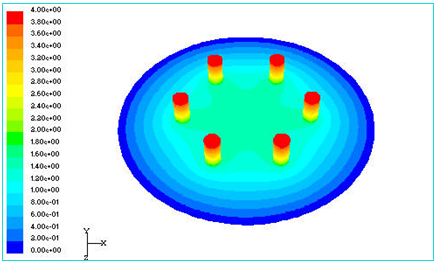
\includegraphics[width=0.5\textwidth]{figures/pic2-1.png}
    \caption{太合金多炭钢铁产品柱扭曲局部受力分析示意图}
    \label{fig:2-1}
\end{figure}

\textcolor{red}{\textbf{表:}}\par
表应具有“自明性”。\par
表应有编号。表的编号由“表”和从“1”开始的阿拉伯数字组成,表较多时,可分章编号。表较多时,可分章编号。\par
表宜有表题,表题即表的名称,置于表的编号之后。表的编号和表题应置于表上方。\par
表的编排,一般是内容和测试项目由左至右横读,数据依序竖读。\par
表的编排建议采用国际通行的三线表。\par
如某个表需要转页接排,在随后的各页上应重复表的编号。编号后跟表题(可省略)和“(续)”,置于表上方。\par
续表均应重复表头。\par
表格示例1:

\begin{table}[htbp]

    \centering
    \caption{国际单位制的基本单位}
    \label{tbl:2-1}
    \begin{tabularx}{0.8\textwidth}{*{3}{>{\centering\arraybackslash}X}}
        \toprule
        量的名称   & 单位名称     & 单位符号 \\ \midrule
        长度       & 米           & m        \\
        质量       & 千克(公斤)   & kg       \\
        时间       & 秒           & s        \\
        电流       & 安{[}培{]}   & A        \\
        热力学温度 & 开{[}尔文{]} & K        \\
        物质的量   & 摩{[}尔{]}   & mol      \\
        发光强度   & 坎{[}德拉{]} & cd       \\ \bottomrule
    \end{tabularx}
\end{table}

\textcolor{red}{\textbf{公式:}}\par
论文中的公式应另行起,并缩格书写,与周围文字留足够的空间区分开。\par
如有两个以上的公式,应用从“1”开始的阿拉伯数字进行编号,并将编号置于括号内。公式的编号右端对齐,公式与编号之间可用“…”连接。公式较多时,可分章编号。\par
公式示例1:
\begin{equation}
    \label{eqn:2}
    \phi=\frac{D_{p}^{2}}{150} \frac{\psi^{3}}{(1-\psi)^{2}}
\end{equation}
\begin{equation}
    \label{eqn:3}
    C_{2} =\frac{3.5}{D_{p}} \frac{(1-\psi)}{\psi^{3}}
\end{equation}

\noindent 式中  $\quad D_{p}$ —— 多孔质材料的平均粒子直径($m$);\par
$\psi$ —— 孔隙度(孔隙体积占总体积的百分比); \par
$\phi$ —— 特征渗透性或固有渗透性,与材料的结构性质有关($m^2$)。\par
较长的公式需要转行时,应尽可能在“=”处回行,或者在“+”、“-”“×”、“/”等记号处回行。\par
公式中分数线的横线,其长度应等于或略大于分子和分母中较长的一方。\par
如正文中书写分数,应尽量将其高度降低为一行。如将分数线书写为“/”,将根号改为负指数。\par
\newpage
公式示例2:\par
\begin{spacing}{2}
    \begin{math}
        \zihao{5} \quad\text{将}\;\dfrac{1}{\sqrt{2}}\;\text{写成}\; 1/\sqrt{2} \;\text{或}\; 2^{-1/2}。
    \end{math}
\end{spacing}

\textcolor{red}{\textbf{引文标注}}\par
论文中引用的文献的标注方法遵照GB/T 7714-2005,可采用顺序编码制,也可采用著者-出版年制,但全文必须统一。\par
\textcolor{red}{\textbf{注释}}\par
当论文中的字、词或短语,需要进一步加以说明,而又没有具体的文献来源时,用注释。注释一般在社会科学中用得较多。\par
应控制论文中的注释数量,不宜过多。\par
由于论文篇幅较长,建议采用文中编号加“脚注”的方式。最好不用采用文中编号加“尾注”。\par

\section{【2级标题,小三号黑体字】 }
 [鼠标左键单击选择该段落,输入替换之。内容为小四号宋或楷体字。]
\subsection{【3级标题,四号黑体字】 }
[鼠标左键单击选择该段落,输入替换之。内容为小四号宋或楷体字。]
\chapter{算法实现}
\markboth{正文}{正文}

第一章的分析指出,现有研究已经证明了单目深度估计在改善深度图像超分辨率重建性能方面的有效性,但不足的是并没有明确地探究两个任务的相关性。与之前的工作不同,本文提出了单目深度估计和深度图像超分辨率重建的联合学习网络(BridgeNet),以实现更好的深度图像超分辨率重建性能。

本文提出的联合学习网络是基于第二章所陈述的理论和技术构建的,本章将按照自顶向下的逻辑,由网络的整体到局部分层进行介绍。首先将介绍本文提出的单目深度估计和深度图像超分辨率重建的联合学习网络(BridgeNet)的网络架构及训练策略,然后将介绍用于子网络间交互的桥接器的设计动机和模块功能。

\section{网络架构}

图 \ref{fig:fig3-1} 描述了本文提出的单目深度估计和深度图像超分辨率重建联合学习网络(BridgeNet)的总体架构,该网络由两个子网络(即深度图像超分辨率重建子网络和单目深度估计子网络)和两个桥接器(即高频注意力桥和内容引导桥)组成。将深度图像超分辨率重建子网络(DSRNet)和单目深度估计子网络(MDENet)集成到一个统一的框架中,以实现深度图像超分辨率重建和单目深度估计的联合学习,并分别将高频注意力桥(HABdg)和内容引导桥(CGBdg)应用于网络的编码器和解码器,以将这两个任务桥接在一起。

\begin{figure}[!htbp]
%	\vspace{-0.8cm}  %调整图片与上文的垂直距离
	\centering
	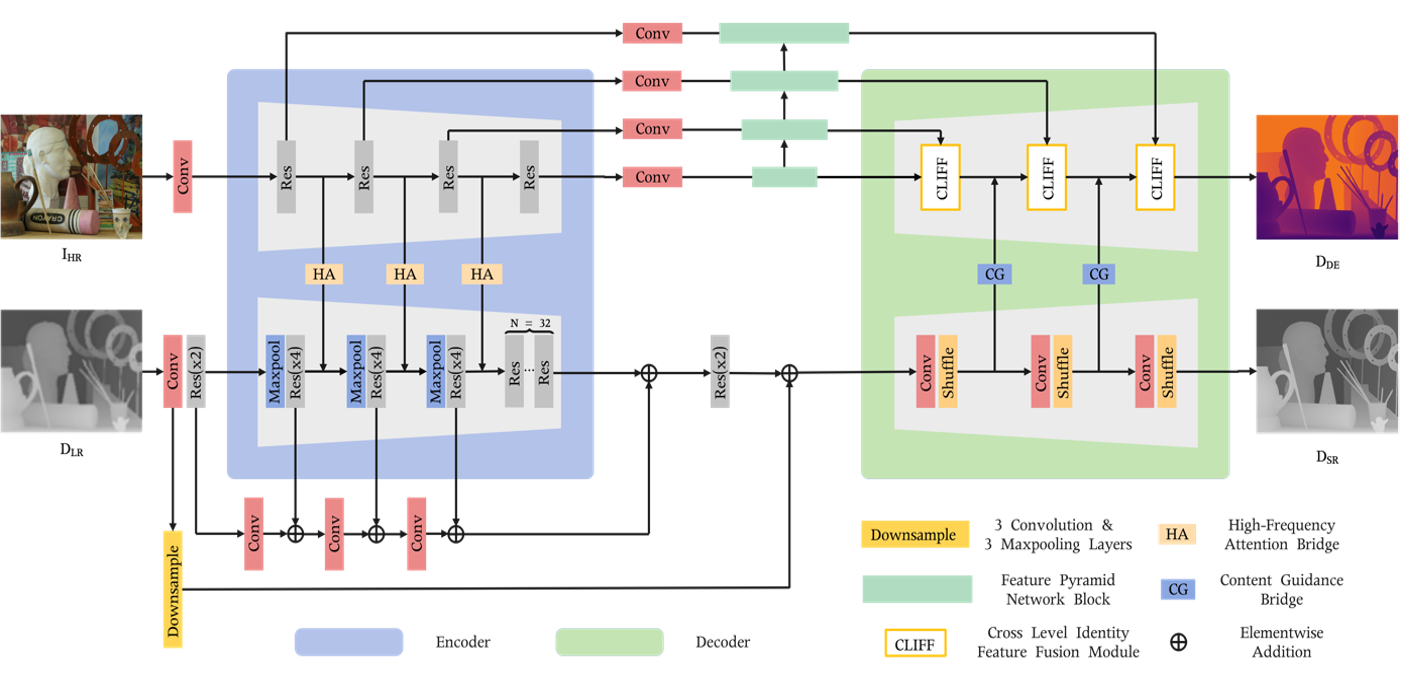
\includegraphics{figures/17.png}
	\caption{单目深度估计和深度图像超分辨率重建联合学习网络(BridgeNet)架构}
	\label{fig:fig3-1}
	\vspace{-0.8cm}  %调整图片与下文的垂直距离
\end{figure}

\newpage
给定一组高分辨率的 RGB-D 图像对 $\{I_{HR}^{\left(n\right)},D_{HR}^{\left(n\right)}\}_{n=1}^N$ 和相应的低分辨率深度图像 $\{D_{LR}^{\left(n\right)}\}_{n=1}^N$ 作为训练数据,其中 $N$ 是训练图像的数量。此外,低分辨率深度图像在输入网络前被插值到高分辨率深度图像的大小。本文提出的网络以低分辨率深度图像($D_{LR}$)和相应的高分辨率彩色图像($I_{HR}$)作为输入,同时对深度图像超分辨率重建子网络和单目深度估计子网络进行训练。超分辨的深度图像($D_{SR}$)是本文网络的主要输出,此外,估计的深度图像($D_{DE}$)也作为辅助输出。

\subsection{单目深度估计子网络}

编码器-解码器(Encoder-Decoder)结构在单目深度估计任务上取得了巨大的成功。本文遵循现有工作 \cite{DBLP:conf/eccv/WangZWLR20} 中使用的编码器-解码器网络结构作为本文联合学习网络的单目深度估计子网络,该子网络由三个部分组成,即特征提取器,特征金字塔网络和深度预测模块。

特征提取器从输入的彩色图像中提取出多种分辨率的多级特征图的集合。然后,通过横向连接将生成的特征图馈送到特征金字塔网络中。特征金字塔网络将提取的语义信息从高层特征传播到低层特征,进而生成优化后的多级特征,即特征金字塔。深度预测模块基于特征金字塔完成最终的深度估计。本文采用经过预训练的 ResNet-50 网络的前5层作为单目深度估计子网络的特征提取器。

为了充分利用特征金字塔,现有的一些方法采用直接融合的策略。在这种策略的指导下,首先将特征金字塔中的所有特征图上采样到相同的分辨率,然后级联在一起用于估计深度图像。尽管具有丰富语义信息的高层特征所估计的深度图像鲁棒性更强,但从非常低的分辨率直接对它们进行上采样,会由于上采样特征图的模糊而导致所估计的深度图像也很模糊。

另一种策略是对特征金字塔中不同分辨率的特征渐进式地融合。这种方法首先对高层特征进行逐步上采样,然后与相同分辨率的低层特征进行融合。虽然这样的融合方式可以在一定程度上抑制在深度估计时的模糊问题,但其输出特征主要受低级特征所决定,而这样的特征对于较难估计的场景并不具有鲁棒性。

在本文的单目深度估计子网络特征解码期间,跨层恒等特征融合(Cross-level Identity Feature Fusion, CLIFF)模块用于逐步融合优化的多层特征并完成深度估计,其结构如图 \ref{fig:fig3-2} 所示。跨层恒等特征融合模块以高层特征图和低层特征图作为输入。首先使用双线性插值(Bilinear Interpolation)将高层特征图进行上采样,使得输入的两个特征图具有相同的分辨率。由于高层特征具有丰富的语义信息且噪声更少,因此借用注意力机制的思想,通过将低层特征与高层特征相乘来对低层特征进行强化。如此一来,低层特征中的准确响应得到进一步的增强,而噪声响应则会受到抑制。为了得到高层特征、原始的和强化后的低层特征的最佳组合,跨层恒等特征融合模块通过两个卷积层来对三个特征进行进一步选择。

\begin{figure}[!htbp]
%	\vspace{-0.8cm}  %调整图片与上文的垂直距离
	\centering
	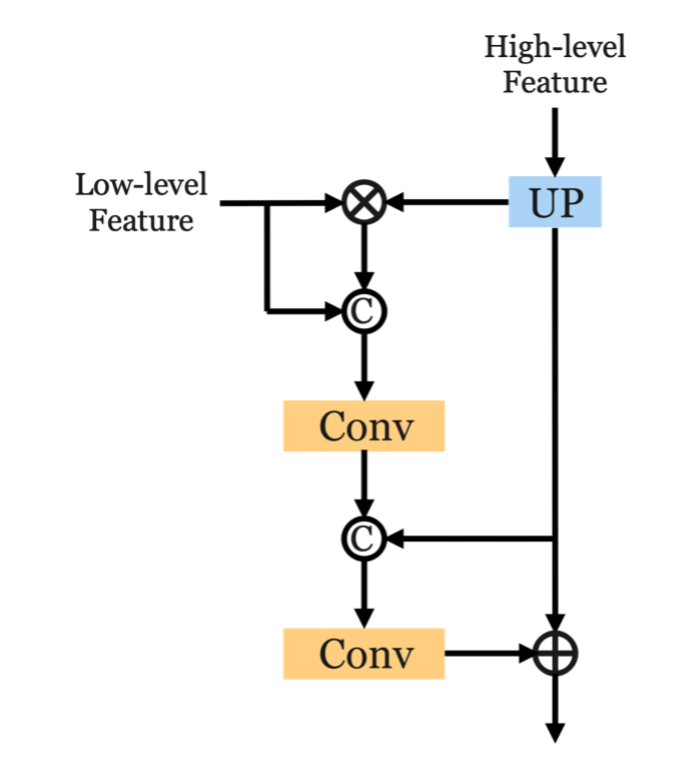
\includegraphics{figures/18.png}
	\caption{跨层恒等特征融合模块结构图}
	\label{fig:fig3-2}
	\vspace{-0.8cm}  %调整图片与下文的垂直距离
\end{figure}

具体而言,原始的低层特征和强化后的低层特征在级联后将作为第一个卷积层的输入,而第一个卷积层用于学习从级联的特征中提取更有用的信息。其输出将与高级特征级联起来,用作第二个卷积层的输入,从而实现对低层特征和高层特征的选择与聚合。此外,出于保留高级语义特征的考虑,在上采样的高层特征与第二个卷积层的输出特征之间添加了恒等映射(Identity Mapping)。通过跨层恒等特征融合模块得到的特征,兼顾了高层特征的语义信息和低层特征的结构信息,是对单目深度估计最有利的特征组合。
跨层恒等特征融合模块中所进行的操作可以描述为式 \ref{equ:equ3-1} 至式 \ref{equ:equ3-4}。

\begin{equation}
	F^a=F^l\odot F^h
	\label{equ:equ3-1}
\end{equation}
\vspace{-0.8cm}
\begin{equation}
	F_1^c=W_1\left(\left[F^l,F_a\right]\right)
	\label{equ:equ3-2}
\end{equation}
\vspace{-0.8cm}
\begin{equation}
	F_2^c=W_2\left(\left[F_1^c,F^h\right]\right)
	\label{equ:equ3-3}
\end{equation}
\vspace{-0.8cm}
\begin{equation}
	F^o=F_2^c+F^h
	\label{equ:equ3-4}
\end{equation}

\noindent 式中,$F^l$,$F^a$,$F^h$ —— 原始的和强化后的低层特征及高层特征;\newline
 \indent\quad $F_1^c$,$F_2^c$,$F^o$ —— 两个卷积层的输出及最终输出;\newline
 \indent\quad $W_1$,$W_2$ —— 两个卷积层的权重;\newline
 \indent\quad $\odot$ —— 像素级相乘;\newline
 \indent\quad $[·,·]$ —— 级联操作。
 
 \newpage
 
 \subsection{深度图像超分辨率重建子网络}
 
 遵循人脸超分辨率网络的结构 \cite{DBLP:conf/aaai/YinRZF20},本文同样将编码器-解码器网络作为深度图像超分辨率重建的基线。其中,编码器由一个浅层特征提取器(包含一个卷积层和一个残差块)和三个连续的特征编码模块以及一些堆叠的残差块构成。每个特征编码模块由一个最大池化层和四个串联的残差块组成,残差块的结构如图 \ref{fig:fig3-3} 所示。最大池化层可以确保深度图像超分辨率重建子网络编码器每一层的特征与单目深度估计子网络编码器对应层特征的分辨率相同,以便后续特征指导的顺利进行。

\begin{figure}[!htbp]
%	\vspace{-0.8cm}  %调整图片与上文的垂直距离
	\centering
	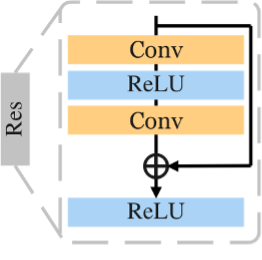
\includegraphics{figures/19.png}
	\caption{残差模块结构图}
	\label{fig:fig3-3}
	\vspace{-0.8cm}  %调整图片与下文的垂直距离
\end{figure}

在深度图像超分辨率重建子网络中,所有卷积层都使用大小相同的 $3 \times 3$ 卷积核,且每个卷积操作后面紧随一个 ReLU 激活函数。除最后的卷积层通道数设置为 3 外,子网络中其余的所有卷积操作的通道数均设置为256。深度图像超分辨率重建子网络所采用的残差模块与原始残差网络的结构基本一致,不同的是移除了残差块中的批量归一化层。

这样做的动机是由于批量归一化层(正则化层)对特征进行了归一化处理,从而导致网络丢弃了范围灵活性,所以最好是移除这些批量归一化层。现有研究 \cite{DBLP:conf/cvpr/LimSKNL17} 的实验也表明用于图像超分辨率重建的残差网络在去除所有的批量归一化层后表现最佳。不仅如此,批量归一化层会减慢网络收敛的速度,同时降低其整体性能,尤其是在图像的超分辨率重建任务中。因此在深度图像超分辨率重建子网络中,所有残差模块中的批量归一化层都被移除。

更深层的网络已经在包括图像超分辨率重建在内的许多计算机视觉任务中显示出更好的性能。增加网络的深度也是现有许多工作中使用的一种策略。经过三个特征编码模块提取出的特征将传递到由 $N$ 个残差块组成的更深层的特征提取模块中。较深的网络可以帮助超分辨的深度图像恢复出更分明的边缘和形状。
\newpage
为了恢复深度图像中的精细结构和微小物体,本文引入了多尺度策略,通过进一步融合深度图像超分辨率重建子网络编码器中间层的特征来优化高层特征。考虑到相邻层特征的相似性,并非编码器的所有特征都需要参与多尺度特征融合以形成新的特征表示,而是仅仅采用了每个特征编码模块提取的特征进行融合。因此每个最大池化层之前的特征编码模块的输出都需要通过跳连接,与深层特征模块输出的特征融合以形成具有更丰富信息的特征。此外,由于特征图每经过一个最大池化层都进行了2倍的下采样,为了匹配不同层特征图的大小,将步长为2的3×3卷积层应用于由跳连接提供的中间层特征,以实现下采样并进行特征融合。

对于低分辨率的深度图像 $D_{LR}$,上述操作可以被描述为式 \ref{equ:equ3-5} 至式 \ref{equ:equ3-7}。

\vspace{-0.4cm}
\begin{equation}
	F_0=f_0\left(D_{LR}\right)
	\label{equ:equ3-5}
\end{equation}
\vspace{-0.8cm}
\begin{equation}
	F_i=f_i\left(F_{i-1}\right),i\in\{1,2,3\}
	\label{equ:equ3-6}
\end{equation}

\noindent 式中,$F_0$ —— 通过一个卷积层和一个残差块提取的浅层特征;\newline
\indent\quad $F_i$,$i\in\{1,2,3\}$ —— 特征编码模块的输出;\newline
\indent\quad $f_0$ —— 浅层特征提取模块;\newline
\indent\quad $f_i$,$i\in\{1,2,3\}$ —— 特征编码模块。

\vspace{-0.4cm}
\begin{equation}
	F_{fusion}=g_3\left(g_2\left(g_1\left(F_1\right)+F_0\right)+F_2\right)+F_3
	\label{equ:equ3-7}
\end{equation}

\noindent 式中,$F_{fusion}$ —— 多尺度特征融合的输出;\newline
\indent\quad $g_i$,$i\in\{1,2,3\}$ —— 实现对中间层特征下采样的卷积层。

在特征解码期间,本文使用了三个顺序连接的相同上采样模块,包括一个卷积层和一个像素重组层(PixelShuffle)。特征图每经过一个上采样模块后,分辨率都变为之前的两倍。最后应用一个 $1 \times 1$ 的卷积层来重建高分辨率的深度图像。

受彩色图像超分辨率重建算法稠密残差网络(Residual Dense Network, RDN)\cite{DBLP:conf/cvpr/ZhangTKZ018} 的启发,编码器初始阶段提取的浅层特征和输入解码器的特征在进行第一次上采样前通过一个大的跳连接进行融合。设计这个跳连接的目的是为了直接提供深度图像超分辨率重建需要的低频信息,从而迫使网络更加专注于学习重建需要的高频信息而不是已经提供的低频信息。

根据网络的设计可以看到,网络提取的浅层特征图大小与上采样后的低分辨率特征图大小相同。而网络中有3个最大池化层,每个最大池化层对特征图进行因子为 $\times 2$ 的下采样,即特征图在经过编码器中三个最大池化后,分辨率下降为输入图像的1/8。为了保证长跳连接两侧的特征图拥有相同的分辨率,浅层特征被馈送到下采样(Downsample)块中以生成低频特征,然后通过长跳连接与编码器提取的最终特征相融合,下采样块的结构如图 \ref{fig:fig3-4} 所示。

\begin{figure}[!htbp]
%	\vspace{-0.8cm}  %调整图片与上文的垂直距离
	\centering
	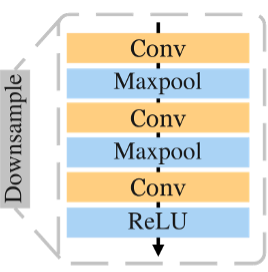
\includegraphics{figures/20.png}
	\caption{下采样模块结构图}
	\label{fig:fig3-4}
	\vspace{-0.8cm}  %调整图片与下文的垂直距离
\end{figure}

\subsection{联合学习策略}
深度图像超分辨率重建和单目深度估计具有天然的相关性,可以在同一数据集的监督下对他们进行训练。因此,这两个任务的联合学习首先体现在损失函数的联合优化上。

与其他多任务学习的损失函数为所有分支损失函数的加权和不同,本文分别为深度图像超分辨率重建和单目深度估计的损失函数分配了不同的优化器。这是因为深度图像超分辨率重建和单目深度估计的学习难度大不相同,导致两个任务的收敛速度不同,从而很难找到合适的权重设置来确保两个任务都达到最佳性能。因此,在损失函数的设计方面,本文提出分别对深度图像超分辨率重建和单目深度估计相关部分进行优化的策略。其损失函数定义为式 \ref{equ:equ3-8} 和式 \ref{equ:equ3-9}。
\vspace{-0.3cm}
\begin{equation}
	\mathcal{L}_{DSR}=||D_{SR}-D_{HR}||_1
	\label{equ:equ3-8}
\end{equation}
\vspace{-0.8cm}
\begin{equation}
	\mathcal{L}_{MDE}=||D_{DE}-D_{HR}||_1
	\label{equ:equ3-9}
\end{equation}

\noindent 式中,$\mathcal{L}_{DSR}$ —— 深度图像超分辨率重建任务的逐像素 $L_1$ 损失;\newline
\indent\quad $\mathcal{L}_{MDE}$ —— 单目深度估计任务的逐像素 $L_1$ 损失。

除了在损失函数层级对两个任务进行约束外,本文还精心设计了两个桥接器,分别将两个任务在编码器和解码器阶段相关联,以实现互利共赢。一个是编码器中的高频注意力桥(HABdg),另一个是解码器中的内容引导桥(CGBdg)。其中,高频注意力桥利用单目深度估计子网络出色的彩色特征学习能力为深度图像超分辨率重建提供指导。考虑到两个任务难度的差异,深度图像超分辨率重建子网络在解码器阶段经由内容引导桥可以为深度估计提供有效的内容指导,从而提高深度估计的性能。在以下各小节中,本文将详细介绍这两个桥接器的设计原理和实现细节。
下面给出深度图像超分辨率重建和单目深度估计联合学习网络训练策略的伪代码。

%\begin{algorithm}[H]
%        \caption{Joint Learning Strategy}
%        \LinesNumbered
%        \KwIn{Training data $D_{LR}$, $I_{HR}$, $D_{HR}$}
%        \KwOut{$D_{SR}$, $D_{DE}$}
%        Randomly initialize DSRNet and MDENet\\
%       
%        \For{ epoch=1; epoch $\leq$ 400;}
%        {
%         ——————————————— Step 1 ———————————————\\
%        $F_{MDE}=Encoder_{MDE}(I_{HR}^n)$\\
%        $F_{DSR}^{shallow}=Res^{(2)}(conv(D_{LR}))$ \tcp*{shallow feature extraction}
%        \For(\tcp*[f]{ i refers to $i^{th}$ layer of encoder}){i=1; i $\leq$ 3} 
%        {
%        \If{i=1}
%        {
%        $Fe_{DSR}^i=maxpool(Res^{(4)}(F_{DSR}^{shallow}))$\\
%        }
%        \Else{
%        $Fe_{DSR}^i=maxpool(Res^{(4)}(F_{ha}^{i-1}))$\\
%        }
%        $F_{blurred}^i=deconv(avgpool(F_{MDE}^i)$\\
%        $A_{hf}^i=PRelu(F_{MDE}^i-F_{blurred}^i)$\\
%        $F_{hg}^i=F_{MDE}^i+A_{hf}^i\cdot F_{MDE}^i$\\
%        $F_{comp}^i=[Fe_{DSR}^i,F_{hg}^i]$\\
%        $F_{ha}^i=SA(conv_{1\times 1}(CA(F_{comp}^i)))$\\
%        }
%        $F_{DSR}^{deeper}=Res^{(32)}(F_{ha}^3)$\\
%        $F_{DSR}^{multi-scale}=conv(conv(conv(Fe_{DSR}^{shallow}+Fe_{DSR}^1)+F_{DSR}^2)+Fe_{DSR}^3)$\tcp*{multi-scale features fusion}
%        $F_{DSR}^{fusion}=Res^{(2)}(F_{DSR}^{deeper}+F_{DSR}^{multi-scale})$\\
%        $F_{DSR}^{low-freq}=Downsample(F_{DSR}^{shallow})$\\
%        \For(\tcp*[f]{ j refers to $j^{th}$ layer of decoder}){i=1; i $\leq$ 3} 
%        {
%        \If{i=1}
%        {
%        $Fd_{DSR}^j=pixelshuffle(conv(F_{DSR}^{fusion}+F_{DSR}^{low-freq}))$\\
%        }
%        \Else{
%        $Fd_{DSR}^j=pixelshuffle(conv(F_{DSR}^{j-1}))$\\
%        }
%        }
%        $D_{SR}=conv_{1 \times 1}(Fd_{DSR}^3)$\\
%        Update weights of parts related to DSR with $\mathcal{L}_{DSR}=||D_{SR}-D_{HR}||_1$\\
%        ——————————————— Step 2 ———————————————\\
%        $F_{MDE}=Encoder_{MDE}(I_{HR}^n)$\\
%        \For{k=1;k $\leq$ 4}
%        {
%        \If{k=1}
%        {
%        $Fp_{MDE}^k=conv(Fe_{MDE}^{5-k})$
%        }
%        \Else
%        {
%        $Fe_{MDE}^{5-k}=interpolate(Fe_{MDE}^{5-k})$\\
%        $Fp_{MDE}^k= conv(Fe_{MDE}^{5-k} +Fe_{MDE}^{5-(k+1)})$
%        }
%        }
%         
%        \For{j=1;k $\leq$ 3}
%        {
%        \If{j=1}
%        {
%        $Fd_{MDE}^j=CLIFF(Fp_{MDE}^1,Fp_{MDE}^2)$\\
%        }
%        \Else
%        {
%        $M_{DSR}^j=conv_{1\times1}(Fd_{DSR}^j)$\\
%        $M_{MDE}^j=conv_{1\times1}(Fd_{MDE}^j)$\\
%        $W_{diff}^j=softmax(conv_{1\times1}(M_{DSR}^j-M_{MDE}^j))$\\
%        $F_{ca}^j=Fd_{DSR}^j+W_{diff}^j\ast Fd_{DSR}^j$\\
%        $F_{con}^j=[Fd_{MDE}^j,F_{ca}^j]$\\
%        $F_{cg}^j=SA(conv_{1\times1}(CA(F_{con}^j)))$\\
%        $Fd_{MDE}^j=CLIFF(F_{cg}^j,Fp_{MDE}^{j+1})$\\
%        }
%        }
%        $D_{DE}=interpolate(conv_{1\times 1}(Fd_{MDE}^3))$\\
%        Update weights of parts related to MDE with $\mathcal{L}_{MDE}=||D_{DE}-D_{HR}||_1$
%        }
%\end{algorithm}

\begin{figure}[!htbp]
	\centering
	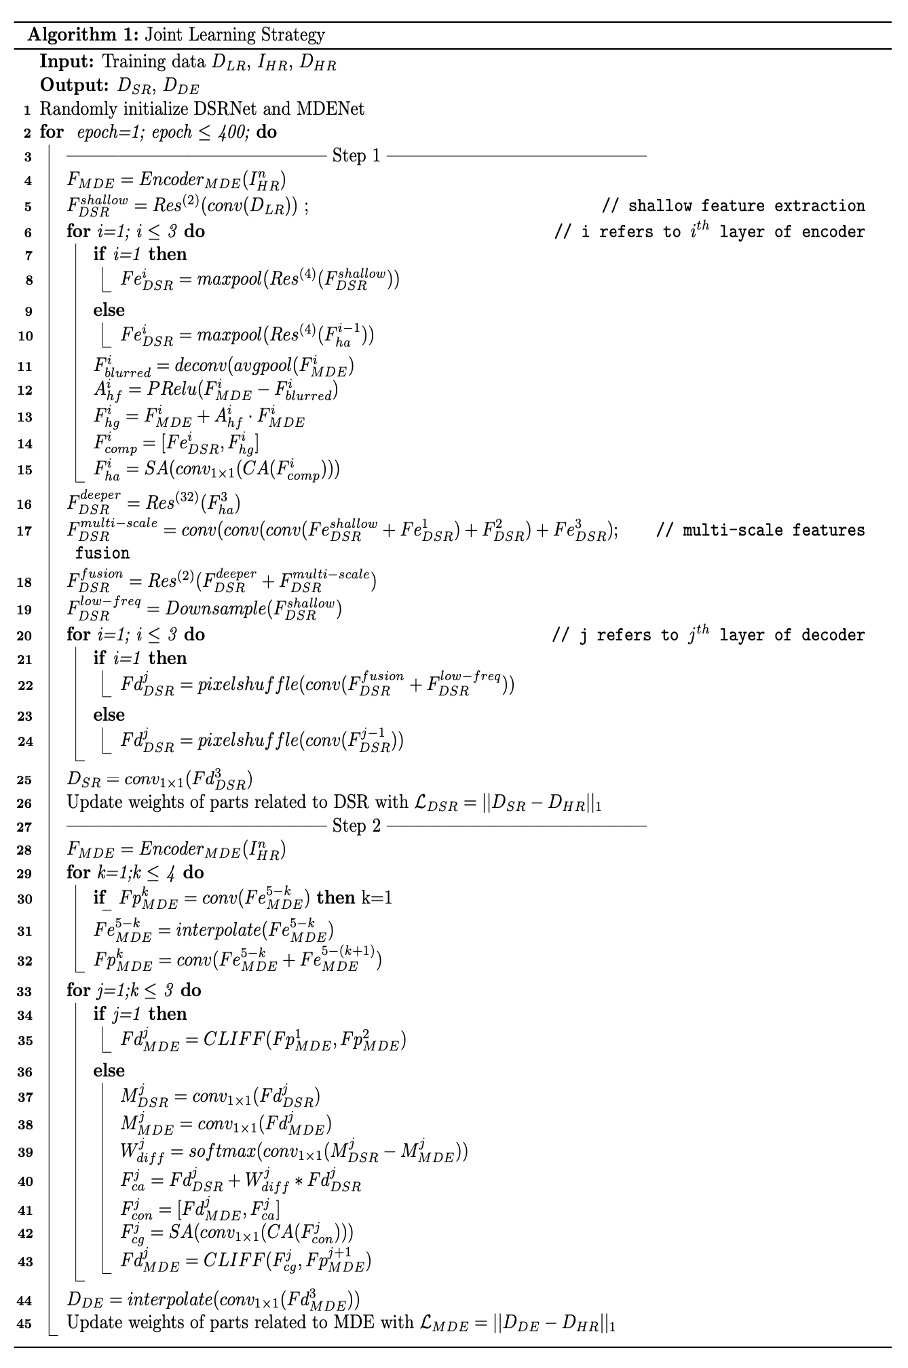
\includegraphics{figures/21.png}
\end{figure}

\section{高频注意力桥}

回顾现有的颜色指导的深度图像超分辨率重建的方法可以发现,彩色图像的指导主要包括对应特征的直接引导 \cite{HuiLT16, LutioDWS19, DBLP:journals/tip/GuoLGCFH19} 或边缘细节的引导 \cite{DBLP:journals/tmm/WangXCZSY20, DBLP:conf/icassp/YeDL18}。尽管彩色图像和深度图像具有很强的结构相似性,但是彩色图像丰富的纹理和边缘并不总是与深度图像一致,因此直接的特征引导或边缘引导可能会导致纹理复制和深度流失等问题。

在联合学习视角下,单目深度估计为解决上述问题提供了新的思路。单目深度估计任务是以彩色图像作为输入,然后实现将场景从光度表示映射到几何表示,从而生成深度图像。因此,由单目深度估计编码器提供的彩色图像的特征更接近于深度模态的特征表示。由单目深度估计编码器为深度图像超分辨率重建任务提供高频信息指导时,可以避免明显的伪影。这就是本文提出在编码器阶段使用单目深度估计代替现有方法的颜色分支来指导深度图像超分辨率重建的原因。

在明确了指导信息的传递方向之后,接下来需要思考的问题便是如何有效地实现。最简单直观的方法是通过级联或相加将单目深度估计子网络相应层的特征直接传递到深度图像超分辨率重建子网络中,但这显然不是明智的方法。在单目深度估计子网络的编码器中,随着网络的深入,特征图的分辨率逐渐降低,其中高层特征具有丰富的语义信息,而低层特征则具有更多的结构信息。由于低分辨率深度图像包含的高频信息较少,因此高分辨率的彩色图像可以为深度图像超分辨率重建提供更为重要的高频信息(例如边缘细节),而不是图像的语义信息。因此,本文设计了一个高频注意力桥,该桥接器用于从单目深度估计子网络学习高频信息以用于指导深度图像超分辨率重建子网络。高频注意力桥的结构如图 \ref{fig:fig3-5} 所示。

\begin{figure}[!htbp]
%	\vspace{-0.8cm}  %调整图片与上文的垂直距离
	\centering
	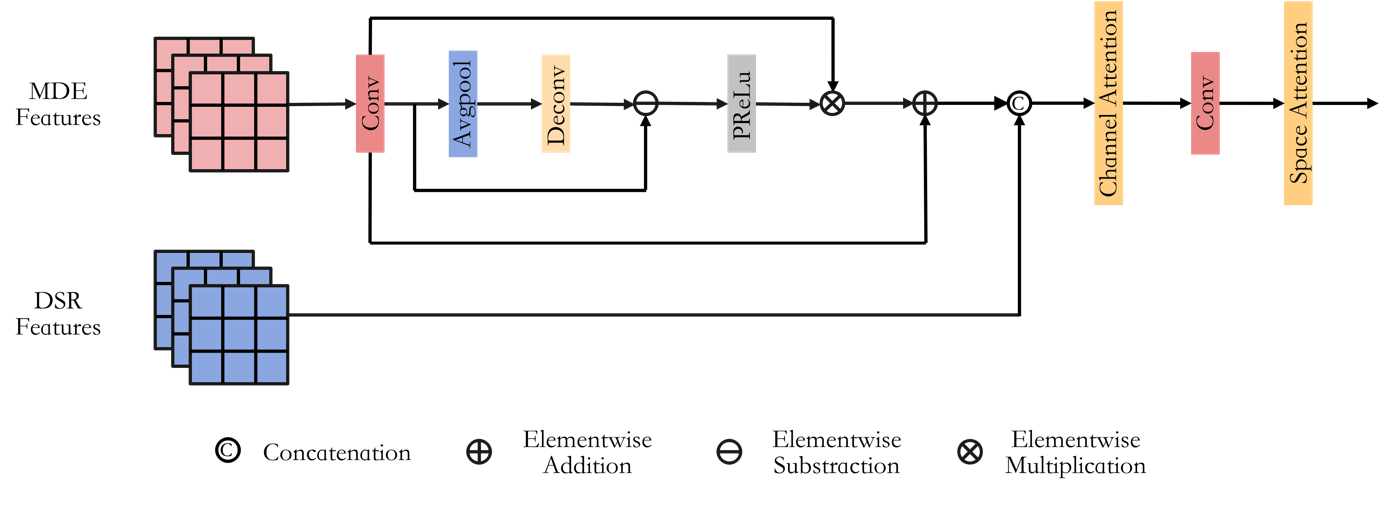
\includegraphics{figures/22.png}
	\caption{高频注意力桥结构图}
	\label{fig:fig3-5}
	\vspace{-0.8cm}  %调整图片与下文的垂直距离
\end{figure}

具体来说,首先使用平均池化和反卷积运算对单目深度估计子网络的原特征进行模糊操作,这一操作可以被描述为式 \ref{equ:equ3-10}。

\begin{equation}
	F_{blurred}^i=deconv\left(avgpool\left(F_{MDE}^i\right)\right)
	\label{equ:equ3-10}
\end{equation}

\noindent 式中,$F_{blurred}^i$ —— 获得的单目深度估计子网络第 $i$ 层的模糊特征;\newline
\indent\quad  $F_{MDE}^i$ —— 单目深度估计子网络第 $i$ 层的特征;\newline
\indent\quad $avgpool\left(\cdot\right)$ —— 平均池化操作;\newline
\indent\quad $deconv\left(\cdot\right)$ —— 反卷积操作。

然后,通过将原始特征与模糊特征相减来获得特征中的高频信息,进而生成高频信息的注意力,即式 \ref{equ:equ3-11}。

\begin{equation}
	A_{hf}^i=PRelu\left(F_{MDE}^i-F_{blurred}^i\right)
	\label{equ:equ3-11}
\end{equation}

\noindent 式中,$A_{hf}^i$ —— 获得的第 $i$ 层的高频注意力;\newline
\indent\quad $PRelu\left(\cdot\right)$ —— 带参数的修正线性单元,即激活函数。

接着,使用获得的高频注意力来对单目深度估计子网络提取的原始特征进行修正和优化,通过残差连接最终得到优化后的引导特征,即式 \ref{equ:equ3-12}。

\begin{equation}
	F_{hg}^i=F_{MDE}^i+A_{hf}^i\cdot F_{MDE}^i
	\label{equ:equ3-12}
\end{equation}

\noindent 式中,$F_{hg}^i$ —— 第 $i$ 层优化后的引导特征。

定义上述操作的原因是要在单目深度估计的原始特征中突显高频信息,以便低分辨率深度图像可以在特征融合时最大化地利用其中的高频信息。

为了利用来自单目深度估计子网络编码器优化后的指导特征,首先将它们与深度图像超分辨率重建子网络编码器相应层的特征在通道维度级联起来,以生成复合特征 $F_{comp}^i$。这种简单的特征融合在空间维度和通道维度上会有很多冗余,因此本文引入了一个注意力块,其中包括一个通道注意力 \cite{DBLP:conf/eccv/WooPLK18} 和一个空间注意力 \cite{DBLP:conf/eccv/WooPLK18} 来增强特征融合能力。通道注意力会学习每个特征通道的重要性,而空间注意会突出显示特征图中的重要位置。上述过程可以表述为式 \ref{equ:equ3-13} 和式 \ref{equ:equ3-14}。

\begin{equation}
	F_{comp}^i=\left[F_{DSR}^i,F_{hg}^i\right]
	\label{equ:equ3-13}
\end{equation}
\vspace{-0.8cm}
\begin{equation}
	F_{ha}^i=SA\left(conv_{1\times1}\left(CA\left(F_{comp}^i\right)\right)\right)
	\label{equ:equ3-14}
\end{equation}

\noindent 式中,$F_{ha}^i$ —— 深度图像超分辨率重建子网络第 $i$ 层融合高频信息的特征;\newline
\indent\quad $F_{DSR}^i$ —— 深度图像超分辨率重建子网络第 $i$ 层的特征;\newline
\indent\quad $CA$ —— 通道注意力;\newline
\indent\quad $SA$ —— 空间注意力;\newline
\indent\quad $conv_{1\times1}$ —— 卷积核大小为 $1\times 1$ 的卷积层;\newline
\indent\quad $\left[\cdot,\cdot\right]$ —— 通道维度的级联。

融合了高频信息的特征 $F_{ha}^i$ 将作为深度图像超分辨率重建子网络编码器下一层的输入。

本文采用的通道注意力模块,主要借鉴了卷积注意力机制模块(CBAM: Convolutional Block Attention Module) \cite{DBLP:conf/eccv/WooPLK18} 中通道注意力模块的设计,如图 \ref{fig:fig3-6} 所示。

\begin{figure}[!htbp]
%	\vspace{-0.8cm}  %调整图片与上文的垂直距离
	\centering
	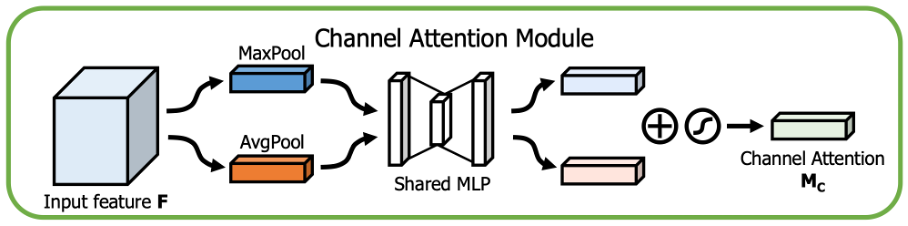
\includegraphics{figures/23.png}
	\caption{通道注意力模块结构图}
	\label{fig:fig3-6}
	\vspace{-0.8cm}  %调整图片与下文的垂直距离
\end{figure}

对于多通道特征图而言,其每一个通道都可以看作是一个独立的“特征”,因此通道注意力关注的是“对于图像而言什么特征是重要的”。为了降低学习通道注意力时的计算开销,最常用的方法是对特征图的空间维度进行“压缩”,现有的大多数工作通常只采用平均池化来聚合特征图的空间信息(如压缩-激励网络)。除平均池化外,最大池化也可用于聚合特征图所蕴含的空间信息,不同的是在梯度下降时平均池化对特征图上每一个像素点都有反馈,而最大池化只对特征图中响应最大的位置有反馈。实验表明最大池化可以挖掘到图像特征的其他重要“线索”,因而可以与平均池化合作学习得到更加有效的通道注意力。因此,本文同时使用平均池化和最大池化来对特征图的空间信息进行压缩,生成两个不同的上下文描述 $F_{avg}^c$ 和 $F_{max}^c$,然后将他们输入到一个共享的网络,并对网络的输出逐像素求和,最后经过 Sigmoid 激活函数以生成通道注意力。整个过程可以描述为式 \ref{equ:equ3-15}。

\begin{equation}
\begin{aligned}
	A^C\left(F\right)&=\sigma\left(MLP\left(AvgPool\left(F\right)\right)+MLP\left(MaxPool\left(F\right)\right)\right)\\
	&=\sigma\left(W_1\left(W_0\left(F_{avg}^c\right)\right)+W_1\left(W_0\left(F_{max}^c\right)\right)\right)
\end{aligned}
\label{equ:equ3-15}
\end{equation}

\noindent 式中,$A^C\left(F\right)$ —— 通道注意力;\newline
\indent\quad $\sigma$ —— Sigmoid 激活函数;\newline
\indent\quad $MLP$ —— 共享的网络;\newline
\indent\quad $AvgPool$ —— 平均池化操作;\newline
\indent\quad $MaxPool$ —— 最大池化操作;\newline
\indent\quad $F$ —— 特征图;\newline
\indent\quad $W_0$,$W_1$ —— 共享网络的权重。

本文采用的空间注意力模块,主要借鉴了卷积注意力机制模块(CBAM: Convolutional Block Attention Module)\cite{DBLP:conf/eccv/WooPLK18} 中空间注意力模块的设计,如图 \ref{fig:fig3-7} 所示。空间注意力是基于像素之间的空间关系产生的。与通道注意力不同,空间注意力关注的是“对于图像而言哪些位置是重要的”。类似地,本文采用平均池化和最大池化来对特征图的通道维度进行压缩,从而生成两个通道数为 1 的特征图 $F_{avg}^s$ 和 $F_{max}^s$,分别代表原始特征所有通道的平均响应和最大响应。然后将它们级联起来并通过卷积核大小为 $7\ \times 7$ 的卷积层,最后经过 Sigmoid 激活函数以生成空间注意力。

\begin{figure}[!htbp]
%	\vspace{-0.8cm}  %调整图片与上文的垂直距离
	\centering
	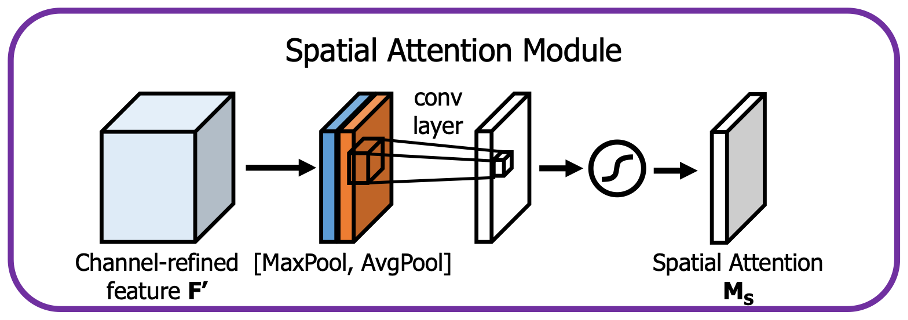
\includegraphics{figures/24.png}
	\caption{空间注意力模块结构图}
	\label{fig:fig3-7}
	\vspace{-0.8cm}  %调整图片与下文的垂直距离
\end{figure}

整个过程可以描述为式 \ref{equ:equ3-16}。

\begin{equation}
\begin{aligned}
	A^S\left(F\right)&=\sigma\left(f^{7\times7}\left([AvgPool\left(F\right);\ MaxPool\left(F\right)\right)\right)\\
	&=\sigma(f^{7\times 7}([F_{avg}^s; F_{max}^s])
\end{aligned}
\label{equ:equ3-16}
\end{equation}

\noindent 式中,$A^S\left(F\right)$ —— 空间注意力;\newline
\indent\quad $\sigma$ —— Sigmoid 激活函数;\newline
\indent\quad $f^{7\times7}$ —— 卷积核大小为 $7 \times 7$ 的卷积层;\newline
\indent\quad $AvgPool$ —— 平均池化操作;\newline
\indent\quad $MaxPool$ —— 最大池化操作;\newline
\indent\quad $F$ —— 特征图。

\section{内容引导桥}

在特征解码阶段,深度图像超分辨率重建子网络和单目深度估计子网络解码器的作用是进一步提取面向任务的特征,以完成深度估计和深度图像的超分辨率重建,最终可以从两个子网络获得相应的估计或超分辨重建的深度图像。两个任务相较而言,单目深度估计由于尺度模糊性 \cite{DBLP:conf/nips/EigenPF14} 而被广泛认知为不适定的逆问题。例如,世界上观察到的许多三维场景可以对应于完全相同的二维平面,即三维场景与二维平面之间是多对一的关系,如图 \ref{fig:fig3-8} 所示。在人眼或相机的成像过程中,大而远的物体和小而近的物体在同一成像平面上的二维信息是一致的,其前提是大物体和小物体具有相同的外观。一个很极端的例子便是现实的房间和其缩小后的展示模型。也就是说在丢失了深度信息后,想要从二维图像推理出场景的真实深度是有很大难度的,这便是尺度模糊性。

\begin{figure}[!htbp]
%	\vspace{-0.8cm}  %调整图片与上文的垂直距离
	\centering
	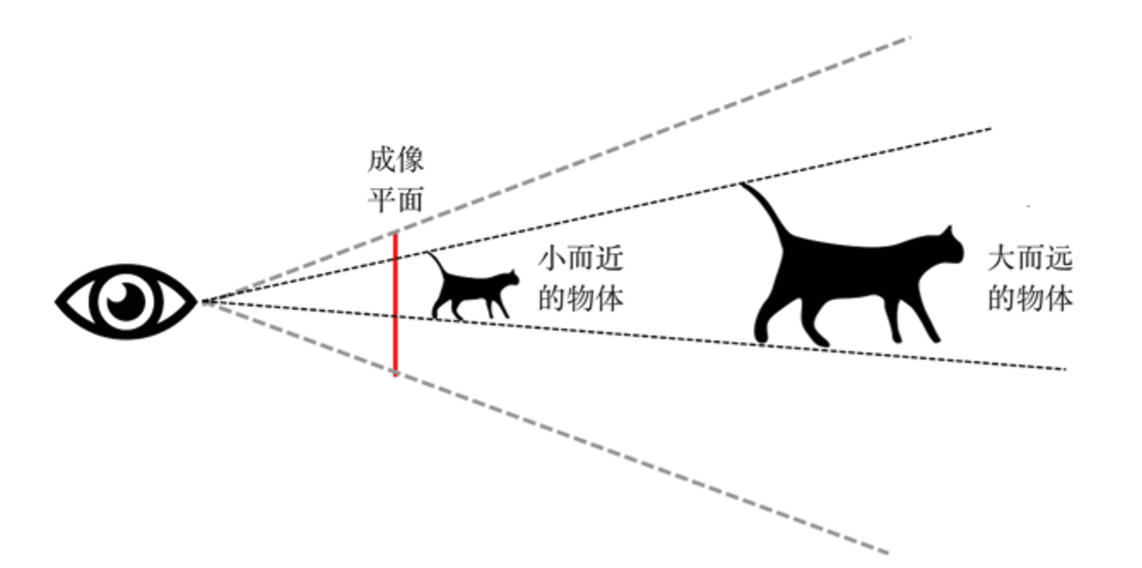
\includegraphics{figures/25.png}
	\caption{尺度模糊性示例图}
	\label{fig:fig3-8}
	\vspace{-0.8cm}  %调整图片与下文的垂直距离
\end{figure}

因此,训练一个可以很好地从彩色图像映射到深度图像的模型是一项非常艰巨的任务。尽管深度图像超分辨率重建也是一个不适定的问题,但它仍在相同的域中学习映射关系并专注于还原图像的细节,故其相对单目深度估计而言更简单。因此,由于两个任务的性能之间存在较大差距,单目深度估计子网络的解码器生成的特征不再适合为深度图像超分辨率重建的解码器提供指导信息。遵循简单任务指导困难任务的原则,本文在解码阶段交换了两个子网络的指导身份,即让深度图像超分辨率重建子网络在深度特征空间为单目深度估计子网络提供内容引导。详细结构如图 \ref{fig:fig3-9} 所示。

\begin{figure}[!htbp]
%	\vspace{-0.8cm}  %调整图片与上文的垂直距离
	\centering
	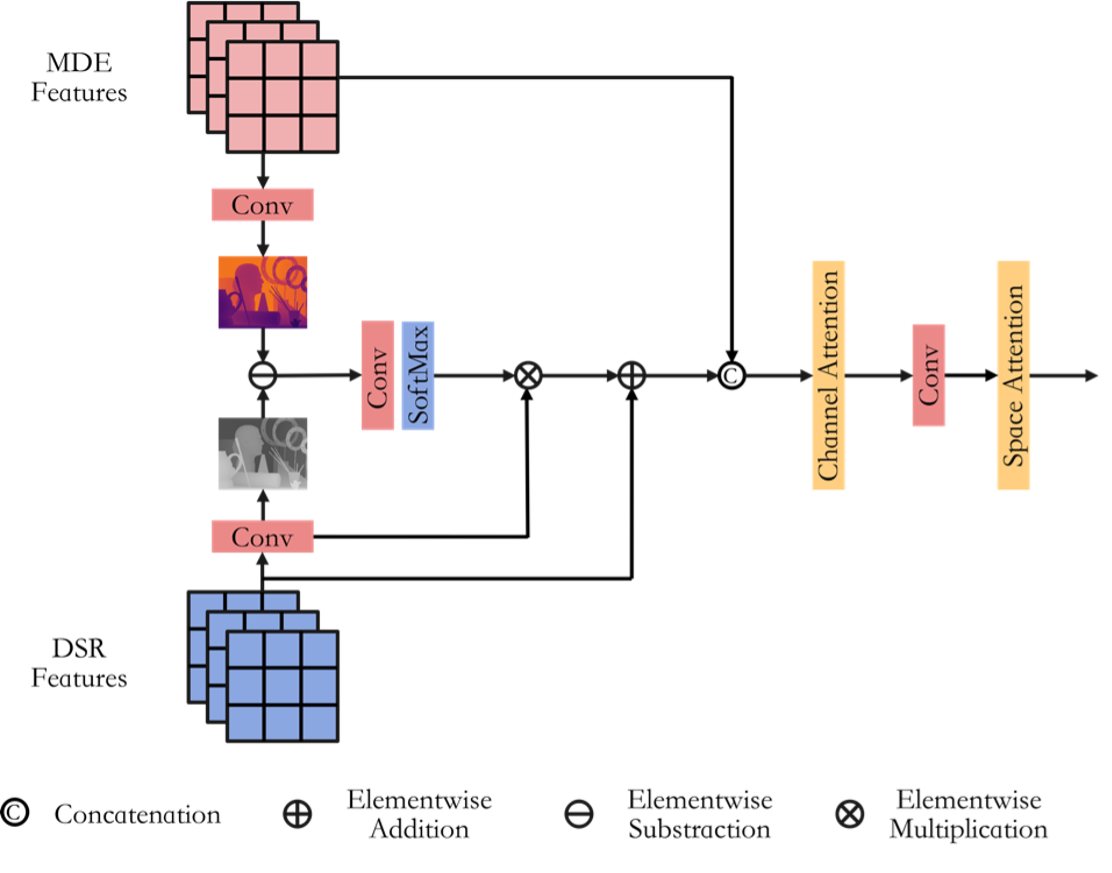
\includegraphics{figures/26.png}
	\caption{内容引导桥结构图}
	\label{fig:fig3-9}
	\vspace{-0.8cm}  %调整图片与下文的垂直距离
\end{figure}

\newpage

如前所述,本文提出的模型可以通过两个子网络的解码器特征获得相应的深度图像。具体来说,本文采用卷积核大小为 $1\times 1$ 的卷积层分别作用于深度图像超分辨率重建子网络和深度估计子网络的解码器,从而获得超分辨率的深度图像和估计的深度图像,即式 \ref{equ:equ3-17} 和式 \ref{equ:equ3-18}。

\vspace{-0.6cm}
\begin{equation}
	M_{DSR}^i=conv_{1\times1}\left(Fd_{DSR}^i\right)
		\label{equ:equ3-17}
\end{equation}
\vspace{-0.8cm}
\begin{equation}
	M_{MDE}^i=conv_{1\times1}\left(Fd_{MDE}^i\right)
	\label{equ:equ3-18}
\end{equation}

\noindent 式中,$M_{DSR}^i$ —— 深度图像超分辨率重建子网络第 $i$ 层生成的深度图像;\newline
\indent\quad $M_{MDE}^i$ —— 单目深度估计子网络第 $i$ 层估计的深度图像;\newline
\indent\quad $Fd_{DSR}^i$ —— 深度图像超分辨率重建子网络解码器第 $i$ 层的特征;\newline
\indent\quad $Fd_{MDE}^i$ —— 单目深度估计子网络解码器第 $i$ 层的特征。

然后,可以计算得到估计的深度图像 $M_{MDE}^i$ 与超分辨率重建的深度图像 $M_{DSR}^i$ 之间的差异图。差异图突出显示了估计的深度图像中相对于超分辨重建的深度图像需要进一步优化的位置,并希望这种差异会随着网络的训练越来越小。在此基础上,本文通过对差异图应用卷积运算和 softmax 激活来学习差异权重,从而为单目深度估计子网络提供内容引导。上述操作可以被描述为式 \ref{equ:equ3-19} 和式 \ref{equ:equ3-20}。

\vspace{-0.4cm}
\begin{equation}
	W_{diff}^i=softmax\left(conv_{1\times1}\left(M_{DSR}^i-M_{MDE}^i\right)\right)
		\label{equ:equ3-19}
\end{equation}
\vspace{-0.8cm}
\begin{equation}
	F_{cg}^i=Fd_{DSR}^i+W_{diff}^i\ast Fd_{DSR}^i
	\label{equ:equ3-20}
\end{equation}

\noindent 式中,$W_{diff}^i$ —— 差异权重;\newline
\indent\quad $F_{cg}^i$ —— 第 $i$ 层的内容引导特征;\newline
\indent\quad $softmax$ —— softmax 激活函数。

最后,本文使用与高频注意力桥中相同的注意力块(包含一个通道注意力和空间注意力)来优化级联的特征(即,$F_{con}^i=\left[Fd_{MDE}^i,F_{cg}^i\right]$),优化后的特征将作为单目深度估计子网络解码器中下一层 CLIFF 模块的高层特征输入,并与来自特征金字塔网络的底层特征进一步融合。

\section{本章小结}

本章从模型的组成和联合学习策略的选择,到深度图像超分辨率重建和单目深度估计两个任务间交互模式的设计进行了详细的介绍。本章介绍了深度图像超分辨率重建和单目深度估计的联合学习网络,以实现更好的深度图像超分辨率重建的性能。与现有工作[22]不同的是,在设计两个子网络之间的交互时,本文采用了更为明确的指导模式。在特征编码器中,单目深度估计子网络通过高频注意力桥为深度图像超分辨率重建子网络提供高频信息的指导。与传统的颜色指导的深度图像超分辨率重建算法相比,单目深度估计子网络提供的颜色指导更接近于深度模态。在特征解码器中,本文遵循简单任务指导困难任务的原则,深度图像超分辨率重建子网络通过内容引导桥为单目深度估计子网络提供内容引导。除了在任务间交互层面的设计外,本章也介绍了在损失函数层级上对两个任务联合优化的策略。


\chapter{实验测试与分析}
\markboth{正文}{正文}

本章将介绍本文提出的单目深度估计和深度图像超分辨率重建联合学习网络在所选择的公开基准数据集上训练和测试取得的效果。第一小节将介绍为验证本文提出的单目深度估计和深度图像超分辨率重建联合学习网络有效性所用到的数据集及选择的评价指标。第二小节将对数据集的训练集和测试集以及具体的参数设置等进行介绍。第三小节将对本文提出的算法在 Middlebury 数据集上取得的结果进行展示并与现有的深度图像超分辨率重建算法进行比较和分析。第四小节将介绍本文提出的算法在 NYU v2 数据集上训练和测试的结果,同样将与现有算法进行比较分析。最后,第五小节通过设计消融实验验证了本文不同模块设计对整体网络性能的影响。

\section{数据集及评价指标}

\subsection{数据集}

\begin{itemize}
	\item[(1)] Middlebury \newline	
	Middlebury 数据集由一系列分别在2001年,2005年,2006年和2014年中引入的子数据集组成。 Middlebury 数据集是在实验室中获取的,其场景仅涵盖不同对象的近景,部分彩色图像和对应的深度图像如图 \ref{fig:fig4-1} 所示。
	
	\begin{figure}[!htbp]
%	\vspace{-0.8cm}  %调整图片与上文的垂直距离
	\centering
	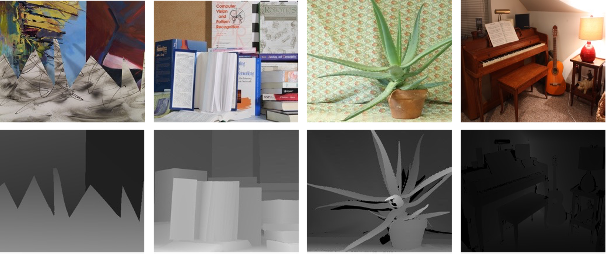
\includegraphics{figures/27.png}
	\caption{Middlebury 数据集彩色图像和深度图像示例}
	\label{fig:fig4-1}
	\vspace{-0.8cm}  %调整图片与下文的垂直距离
\end{figure}

\newpage
\item[(2)] NUY v2 \newline
NYU v2 的原始数据集包含了464个室内场景,是由 RGB-D 摄像机获取的场景的单目视频序列和对应的深度真值。其中,1449个图像对被标注了密集标签且已经对缺失值进行了填充,可以直接用于深度图像超分辨率重建任务。这些带有标签的图像分辨率为 $640 \times 480$,部分彩色图像和对应的深度图像如图 \ref{fig:fig4-2} 所示。

	\begin{figure}[!htbp]
%	\vspace{-0.8cm}  %调整图片与上文的垂直距离
	\centering
	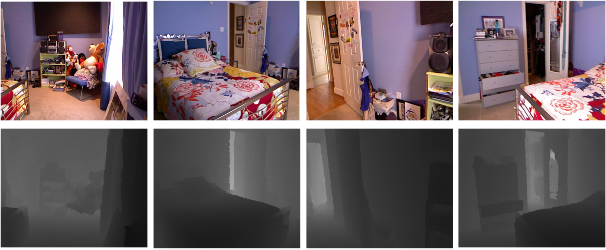
\includegraphics{figures/28.png}
	\caption{NYU v2 数据集彩色图像和深度图像示例}
	\label{fig:fig4-2}
	\vspace{-0.8cm}  %调整图片与下文的垂直距离
	\end{figure}
	
\end{itemize}

\subsection{评价指标}

本文选择了平均绝对差(Mean Absolute Difference, MAD)和均方根误差(Root Mean Square Error, RMSE)来度量超分辨率重建得到的深度图像与真值之间的差异。

对于 Middlebury 数据集 $X=\{I_{HR}^n,D_{HR}^n,D_{LR}^n\}_{n=1}^N$, $I_{HR}^n,D_{HR}^n,D_{LR}^n$ 分别为高分辨率彩色图像和深度图像以及对应的低分辨率深度图像,$N$ 为数据集中图像的数量,则平均绝对差可以定义为式 \ref{equ:equ4-1}。

\begin{equation}
	MAD_{Middlebury}=\frac{1}{N}\sum_{n=1}^{N}\left|D_{HR}^n-SR\left(D_{LR}^n\right)\right|
	\label{equ:equ4-1}
\end{equation}

\noindent 式中,$SR$ —— 超分辨率重建操作。

同样,对于 NYU v2 数据集 $Y=\{I_{HR}^m,D_{HR}^m,D_{LR}^m\}_{m=1}^M$, $I_{HR}^m,D_{HR}^m,D_{LR}^m$ 分别为高分辨率彩色图像和深度图像以及对应的低分辨率深度图像,$M$ 为数据集中图像的数量,则均方根误差可以定义为式 \ref{equ:equ4-2}。

\begin{equation}
	{RMSE}_{NYU\ v2}=\sqrt{\frac{1}{M}\sum_{m=1}^{M}\left(D_{HR}^m-SR\left(D_{LR}^m\right)\right)^2}
	\label{equ:equ4-2}
\end{equation}

\noindent 式中,$SR$ —— 超分辨率重建操作。

\section{实验配置}

本文从 Middlebury 数据集中收集了36对 RGB-D 图像对(分别来自2001 \cite{DBLP:journals/ijcv/BakerSLRBS11},2006 \cite{DBLP:conf/cvpr/HirschmullerS07} 和2014 \cite{DBLP:conf/dagm/ScharsteinHKKNWW14} 的6、21、9张图像)用于训练,将 Middlebury 2005 \cite{DBLP:conf/cvpr/ScharsteinP07} 数据集中的6对 RGB-D 对图像对(分别为 Art,Books,Moebius,Dolls,Laundry,Reindeer)用于测试。本文选取的另一个用于训练和测试的数据集是 NYU v2 数据集 \cite{SilbermanHKF12},并按照通用的划分方法 \cite{DBLP:conf/eccv/LiHA016},将数据集中的前 1000 对 RGB-D 图像对作为训练数据,然后在后449对 RGB-D 图像对上进行评估。此外,用于训练和测试的 RGB-D 图像对被归一在 [0,1] 范围内。

遵循现有工作的方法[10],本文在高分辨率图像输入网络前将其划分为具有重叠的规则网格,即把一幅完整的图像裁剪成足够数量的图像块。这种训练策略不仅不会削弱网络的性能,而且会减少训练的时间。高分辨率的深度图像和彩色图像分别根据 $\times 4$、$\times 8$ 和 $\times 16$ 的上采样因子被裁剪成足够数量(在本文实验中一般裁剪为15000张左右的图像块)的大小为 ${64}^2$、${128}^2$ 和 ${256}^2$ 的图像块。为了获得相应的低分辨率深度图像块,本文使用 Bicubic 插值方法将高分辨率深度图像块下采样为固定大小的 $16 \times 16$ 的图像块。如前文所述,本文引入了平均绝对差(MAD)和均方根误差(RMSE)两个指标,以对模型的性能进行定量评估。

本文提出的网络基于深度学习框架 PyTorch 实现,并使用 NVIDIA 2080Ti GPU 加速训练。在训练期间,一次训练所选取的样本数(Batch Size)为 8。此外,本文选取了动量为 0.9,$\beta_1=0.9$,$\beta_2=0.99$,$\epsilon={10}^{-8}$ 的 ADAM 优化器对训练进行优化。初始学习率设置为 $1e^{-4}$,并且每100轮(epoch)乘以0.1以降低学习速率。在上采样因子为 $\times 8$ 的深度图像超分辨率重建实验中,大小为 $256 \times 256$ 的图像的推理时间为0.052 秒。

\section{基于 Middlebury 数据集的结果比较及分析}

本文在不同上采样因子($\times 4$,$\times 8$ 和 $\times 16$)与一些最新的深度图像超分辨率重建方法进行了比较,包括六种传统深度图像超分辨率重建算法(即 CLMF \cite{LuSMLD12},JGF \cite{0001TT13},TGV \cite{DBLP:conf/iccv/FerstlRRRB13},CDLLC \cite{DBLP:conf/icmcs/XieCFS14},PB \cite{DBLP:conf/eccv/AodhaCNB12} 和 EG \cite{DBLP:journals/tip/XieFS16})和七种基于深度学习的方法(即 SRCNN \cite{DBLP:conf/eccv/DongLHT14}, ATGVNet \cite{DBLP:conf/eccv/RieglerRB16}, MSG \cite{HuiLT16}, DGDIE \cite{DBLP:conf/cvpr/GuZGCCZ17}, DEIN \cite{DBLP:conf/icassp/YeDL18}, CCFN \cite{WenSLLF19}, GSRPT \cite{LutioDWS19}, 和 CTKT \cite{Sun2021cvpr})。

图 \ref{fig:fig4-3} 展示了 $\times 8$ 上采样因子下不同方法在图像 Art 和 Dolls 上的可视化结果比较。其中,(a)为深度图像的真值(Ground Truth)和彩色图像;(b)为低分辨率深度块;(c)-(h)分别为通过 Bicubic,TGV \cite{DBLP:conf/iccv/FerstlRRRB13},MSG \cite{HuiLT16},CTKT \cite{Sun2021cvpr} 和 BridgeNet 超分辨率重建得到的深度图像块;(i)为深度图像的真值图像块。为了获得更加清晰的可视化结果,深度图像块经过了放大。

\newpage
显然,就场景的结构和细节而言,与深度图像的真值相比,本文的方法获得了最相似的重建结果。对于图中的尺寸较大的物体(如 Art 中的茶壶),所有的基于深度学习的方法都呈现出相似的重建结果。然而,对于微小的物体,本文的方法可以恢复深度图像更多的细节。例如,Art 图像中的棍子周围的伪影更少,Doll 图像中的玩具头部轮廓更准确。而其他方法可能会产生一些伪像,边界模糊或形状变化。这些现象与低分辨率深度图像成像时深度相机对精细结构和微小物体的严重破坏有关,从而给这些区域的重建带来了更多困难。因此,本文的方法在准确恢复这些微小物体的深度边界方面更具有优势。

\begin{figure}[!htbp]
%	\vspace{-0.8cm}  %调整图片与上文的垂直距离
	\centering
	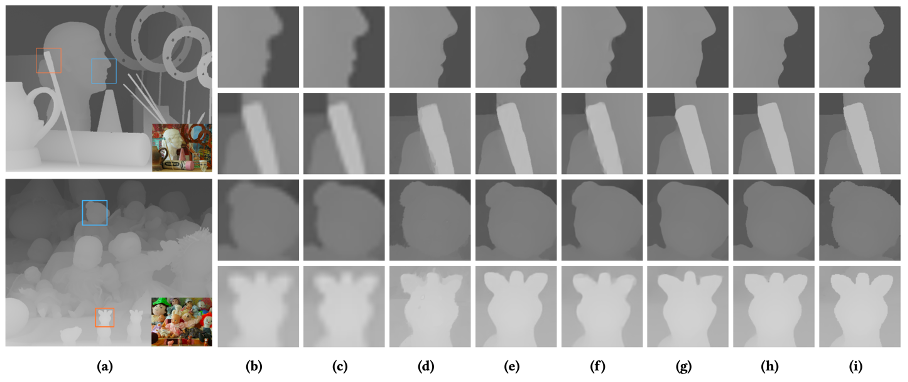
\includegraphics{figures/29.png}
	\caption{Middlebury 数据集 $\times 8$ 不同超分辨率重建方法可视化结果对比}
	\label{fig:fig4-3}
	\vspace{-0.8cm}  %调整图片与下文的垂直距离
	\end{figure}
	
	与其他方法的定量比较如表 \ref{tab:tab4-1} 和表 \ref{tab:tab4-2} 所示(性能最好的模型指标被加粗显示,而性能排名第二的模型指标被下划线标记)。与基于卷积神经网络的方法相比,传统的基于滤波或基于优化的方法具有相对较高的平均绝对差值。而与其他基于卷积神经网络的方法相比,本文提出的单目深度估计和深度图像超分辨率重建联合学习网络(BridgeNet)可以获得具有竞争力的结果,即使在 $\times 8$ 和 $\times 16$ 这样具有挑战性的上采样因子下,本文提出的网络也几乎可以获得最佳的结果。以上采样因子为 $\times 16$ 的深度图像超分辨率重建实验为例,对于 Books 图像,与性能排名第二的算法相比,本文的方法将 MAD 从0.67提升至0.51,百分比增益为23.9%。
	
%\renewcommand{\arraystretch}{0.85}
\setlength{\tabcolsep}{3.5mm}{
\begin{longtable}{c|ccc|ccc|ccc}
\caption{Middlebury 数据集 $\times 8$ 不同超分辨率重建方法量化指标对比(一)}
\label{tab:tab4-1}\\
\toprule[1.5pt]
\multirow{2}{*}{} & \multicolumn{3}{c|}{Art} & \multicolumn{3}{c|}{Books} & \multicolumn{3}{c}{Dolls} \\\cline{2-10}
                  &  $\times 4$      &  $\times 8$      &   $\times 16$    &   $\times 4$      &     $\times 8$   &    $\times 16$    &    $\times 4$     &    $\times 8$    &    $\times 16$    \\\hline
\endfirsthead
\multicolumn{10}{c}%
{\hfill{\zihao{5} 表 \thetable\ (续)}} \\
\toprule[1.5pt]
\multirow{2}{*}{} & \multicolumn{3}{c|}{Art} & \multicolumn{3}{c|}{Books} & \multicolumn{3}{c}{Dolls} \\\cline{2-10}
                  &  $\times 4$      &  $\times 8$      &   $\times 16$    &   $\times 4$      &     $\times 8$   &    $\times 16$    &    $\times 4$     &    $\times 8$    &    $\times 16$    \\\hline
\endhead

CLMF \cite{LuSMLD12}       & 0.76 & 1.44 & 2.87       & 0.28    & 0.51   & 1.02   & 0.34    & 0.60   & 1.01   \\
JGF \cite{0001TT13}        & 0.47 & 0.78 & 1.54       & 0.24    & 0.43   & 0.81   & 0.33    & 0.59   & 1.06   \\
TGV \cite{DBLP:conf/iccv/FerstlRRRB13}        & 0.65 & 1.17 & 2.30       & 0.27    & 0.43   & 0.82   & 0.33    & 0.70   & 2.20   \\
CDLLC \cite{DBLP:conf/icmcs/XieCFS14}     & 0.53 & 0.76 & 1.41       & 0.19    & 0.46   & 0.75   & 0.31    & 0.53   & 0.79   \\\bottomrule[1.5pt]
PB \cite{DBLP:conf/eccv/AodhaCNB12}        & 0.79 & 0.93 & 1.98       & 0.16    & 0.43   & 0.79   & 0.53    & 0.83   & 0.99   \\
EG \cite{DBLP:journals/tip/XieFS16}        & 0.48 & 0.71 & \uline{1.35}     & 0.15    & 0.36   & 0.70   & 0.27    & 0.49   & 0.74  \\\hline
SRCNN \cite{DBLP:conf/eccv/DongLHT14}     & 0.63          & 1.21          & 2.34          & 0.25          & 0.52          & 0.97          & 0.29          & 0.58          & 1.03          \\
ATGVNet \cite{DBLP:conf/eccv/RieglerRB16}   & 0.65          & 0.81          & 1.42          & 0.43          & 0.51          & 0.79          & 0.41          & 0.52          & \textbf{0.56} \\
MSG \cite{HuiLT16}       & 0.46          & 0.76          & 1.53          & 0.15          & 0.41          & 0.76          & 0.25          & 0.51          & 0.87          \\
DGDIE \cite{DBLP:conf/cvpr/GuZGCCZ17}    & 0.48          & 1.20          & 2.44          & 0.30          & 0.58          & 1.02          & 0.34          & 0.63          & 0.93          \\
DEIN \cite{DBLP:conf/icassp/YeDL18}        & 0.40          & 0.64          & \textbf{1.34} & 0.22          & 0.37          & 0.78          & 0.22          & 0.38          & 0.73          \\
CCFN \cite{WenSLLF19}    & 0.43          & 0.72          & 1.50          & 0.17          & 0.36          & 0.69          & 0.25          & 0.46          & 0.75          \\
GSRPT \cite{LutioDWS19}     & 0.48          & 0.74          & 1.48          & 0.21          & 0.38          & 0.76          & 0.28          & 0.48          & 0.79          \\
CTKT \cite{Sun2021cvpr}      & \textbf{0.25} & \textbf{0.53} & 1.44          & \textbf{0.11} & \uline{0.26}    & \uline{0.67}    & \textbf{0.16} & \uline{0.36}    & 0.65          \\
BridgeNet         & \uline{0.30}    & \uline{0.58}    & 1.49          & \uline{0.14}    & \textbf{0.24} & \textbf{0.51} & \uline{0.19}    & \textbf{0.34} & \uline{0.64}   \\
\bottomrule[1.5pt]
\end{longtable}}

\setlength{\tabcolsep}{3.5mm}{
\begin{longtable}{c|ccc|ccc|ccc}
\caption{Middlebury 数据集 $\times 8$ 不同超分辨率重建方法量化指标对比(二)}
\label{tab:tab4-2}\\
\toprule[1.5pt]
\multirow{2}{*}{} & \multicolumn{3}{c|}{Art} & \multicolumn{3}{c|}{Books} & \multicolumn{3}{c}{Dolls} \\\cline{2-10}
                  &  $\times 4$      &  $\times 8$      &   $\times 16$    &   $\times 4$      &     $\times 8$   &    $\times 16$    &    $\times 4$     &    $\times 8$    &    $\times 16$    \\\hline
\endfirsthead
\multicolumn{10}{c}%
{\hfill{\zihao{5} 表 \thetable\ (续)}} \\
\toprule[1.5pt]
\multirow{2}{*}{} & \multicolumn{3}{c|}{Art} & \multicolumn{3}{c|}{Books} & \multicolumn{3}{c}{Dolls} \\\cline{2-10}
                  &  $\times 4$      &  $\times 8$      &   $\times 16$    &   $\times 4$      &     $\times 8$   &    $\times 16$    &    $\times 4$     &    $\times 8$    &    $\times 16$    \\\hline
\endhead

CLMF \cite{LuSMLD12}     & 0.50 & 0.80       & 1.67          & 0.29 & 0.51 & 0.97 & 0.51 & 0.84 & 1.55          \\ 
JGF \cite{0001TT13}      & 0.36 & 0.64       & 1.20          & 0.25 & 0.46 & 0.80 & 0.38 & 0.64 & 1.09          \\ 
TGV \cite{DBLP:conf/iccv/FerstlRRRB13}      & 0.55 & 1.22       & 3.37          & 0.29 & 0.49 & 0.90 & 0.49 & 1.03 & 3.05          \\ 
CDLLC \cite{DBLP:conf/icmcs/XieCFS14}   & 0.30 & 0.48       & 0.96          & 0.27 & 0.46 & 0.79 & 0.43 & 0.55 & 0.98          \\ 
PB \cite{DBLP:conf/eccv/AodhaCNB12}      & 1.13 & 1.89       & 2.87          & 0.17 & 0.47 & 0.82 & 0.56 & 0.97 & 1.89          \\ 
EG \cite{DBLP:journals/tip/XieFS16}      & 0.28 & 0.45       & \uline{0.92}    & 0.23 & 0.42 & 0.75 & 0.36 & 0.51 & 0.95          \\ \hline
SRCNN \cite{DBLP:conf/eccv/DongLHT14}   & 0.40 & 0.87       & 1.74          & 0.25 & 0.43 & 0.87 & 0.35 & 0.75 & 1.47          \\
ATGVNet \cite{DBLP:conf/eccv/RieglerRB16} & 0.37 & 0.89       & 0.94          & 0.38 & 0.45 & 0.80 & 0.41 & 0.58 & 1.01 \\
MSG \cite{HuiLT16}    & 0.30 & 0.46       & 1.12          & 0.21 & 0.43 & 0.76 & 0.31 & 0.52 & 0.99          \\
DGDIE \cite{DBLP:conf/cvpr/GuZGCCZ17}   & 0.35 & 0.86       & 1.56          & 0.28 & 0.58 & 0.98 & 0.35 & 0.73 & 1.29          \\
DEIN \cite{DBLP:conf/icassp/YeDL18}      & 0.23 & \uline{0.36} & 0.81 & 0.20 & 0.35 & 0.73 & 0.26 & 0.40 & 0.80          \\
CCFN \cite{WenSLLF19}   & 0.24 & 0.41       & 0.71          & 0.23 & 0.39 & 0.73 & 0.29 & 0.46 & 0.95          \\
GSRPT \cite{LutioDWS19}   & 0.33 & 0.56       & 1.24          & 0.24 & 0.49 & 0.80 & 0.31 & 0.61 & 1.07          \\
CTKT \cite{Sun2021cvpr}      & \textbf{0.16} & \uline{0.36}    & \uline{0.76}    & \textbf{0.13} & \uline{0.27}    & \uline{0.69}    & \textbf{0.17} & \uline{0.35}    & \uline{0.77}          \\
BridgeNet         & \uline{0.17}    & \textbf{0.34} & \textbf{0.71} & \uline{0.15}    & \textbf{0.26} & \textbf{0.54} & \uline{0.19}    & \textbf{0.31} &  \textbf{0.70}\\
\bottomrule[1.5pt]
\end{longtable}}

\section{基于 NYU v2 数据集的结果比较及分析}

本文还在 NYU v2 数据集上对提出的方法进行评估,并与其他最新的方法进行比较,包括 Bicubic,TGV \cite{DBLP:conf/iccv/FerstlRRRB13}, EDGE \cite{ParkKTBK11}, DJF \cite{DBLP:conf/eccv/LiHA016}, SDF \cite{DBLP:journals/pami/HamCP18}, DGDIE \cite{DBLP:conf/cvpr/GuZGCCZ17}, GbFT \cite{DBLP:conf/iccv/AlbaharH19}, PAC \cite{DBLP:conf/cvpr/SuJSGLK19}, SVLRM \cite{DBLP:conf/cvpr/PanDRLT019}, DKN \cite{DBLP:journals/corr/abs-1903-11286} 和 CTKT \cite{Sun2021cvpr}。

图 \ref{fig:fig4-4} 展示了本文的方法在 $\times 8$ 上采样因子下的可视化结果。其中,(a)为彩色图像;(b)为深度图像真值;(c)-(f)分别为SDF  \cite{DBLP:journals/pami/HamCP18},DJF  \cite{DBLP:conf/eccv/LiHA016},SVLRM  \cite{DBLP:conf/cvpr/PanDRLT019} 和 BridgeNet 超分辨率重建得到的深度图像块。可以看到,无论是在红色矩形区域还是在黄色矩形区域内,本文的方法都可以准确地重建图像的深度信息和微小物体的边缘。如表 \ref{tab:tab4-3} 中所示(性能最好的模型指标被加粗显示,而性能排名第二的模型指标被下划线标记),在 $\times 8$ 和 $\times 16$ 上采样因子的情况下,本文的方法可以获得最佳的性能。与性能排名第二的算法相比,本文方法的 RMSE 在 $\times 8$ 的上采样因子下达到2.63,提升了3.7%。

\begin{figure}[!htbp]
%	\vspace{-0.8cm}  %调整图片与上文的垂直距离
	\centering
	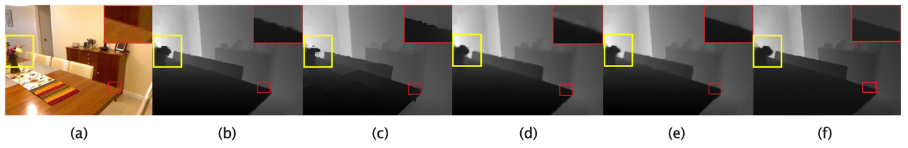
\includegraphics{figures/30.png}
	\caption{NYU v2 数据集 $\times 8$ 不同超分辨率重建方法可视化结果对比}
	\label{fig:fig4-4}
	\vspace{-0.8cm}  %调整图片与下文的垂直距离
	\end{figure}
	
\setlength{\tabcolsep}{14mm}{	
\begin{longtable}{c|ccc}
\caption{NYU v2 数据集 \textbackslash{}times8 不同超分辨率重建方法量化指标对比}
\label{tab:tab4-3}\\
\toprule[1.5pt]
               &     $\times 4$          &         $\times 8$      &        $\times 16$     \\\hline
\endfirsthead
%
\multicolumn{4}{c}%
{\hfill{\zihao{5} 表 \thetable\ (续)}} \\
\toprule[1.5pt]
              &     $\times 4$          &         $\times 8$      &        $\times 16$       \\\hline
\endhead
%
Bicubic       & 8.16          & 14.22         & 22.32         \\
TGV \cite{DBLP:conf/iccv/FerstlRRRB13}    & 6.98          & 11.23         & 28.13         \\
EDGE \cite{ParkKTBK11}   & 5.21          & 9.56          & 18.1          \\
DJF \cite{DBLP:conf/eccv/LiHA016}   & 3.54          & 6.2           & 10.21         \\
SDF \cite{DBLP:journals/pami/HamCP18}   & 3.04          & 5.67          & 9.97          \\
DGDIE \cite{DBLP:conf/cvpr/GuZGCCZ17} & 1.56          & 2.99          & 5.24          \\
GbFT \cite{DBLP:conf/iccv/AlbaharH19}  & 3.35          & 5.73          & 9.01          \\
PAC \cite{DBLP:conf/cvpr/SuJSGLK19}   & 2.39          & 4.59          & 8.09          \\
SVLRM \cite{DBLP:conf/cvpr/PanDRLT019} & 1.74          & 5.59          & 7.23          \\
DKN \cite{DBLP:journals/corr/abs-1903-11286}   & 1.62          & 3.26          & 6.51          \\
CTKT \cite{Sun2021cvpr}  & \textbf{1.49} & \uline{2.73}    & \uline{5.11}    \\
BridgeNet     & \uline{1.54}    & \textbf{2.63} & \textbf{4.98}\\
\bottomrule[1.5pt]
\end{longtable}}
	
\section{消融实验}
在本节中,将进行全面的消融研究以验证单目深度估计和深度图像超分辨率重建联合学习网络(BridgeNet)中的设计对提升深度图像超分辨率重建性能的作用及贡献。表 \ref{tab:tab4-4} 列出了 Middlebury 2005数据集在不同实验设计下进行八倍上采样深度图像超分辨率重建的结果。第一行和第二行是在相同条件下分别单独对深度图像超分辨率重建子网络和单目深度估计子网络训练与测试的结果。从平均绝对差的值来看,单目深度估计子网络的性能不及深度图像超分辨率重建子网络,这样的结果与之前的分析吻合。也就是说,单目深度估计任务的学习难度与深度图像超分辨率重建任务相比较为困难。

对于任务间的交互,本文首先通过简单的损失函数约束将两个任务组合在一起,结果为表 \ref{tab:tab4-4} 的第三行。与单独的深度图像超分辨率重建子网络相比,深度图像超分辨率重建的 MAD 优化到0.363。然后,逐渐将高频注意力桥(HABdg)和内容引导桥(CGBdg)集成到网络中以验证它们的作用。在联合学习网络中仅使用高频注意力桥或内容引导桥时,获得的结果要好于仅使用损失函数约束。此外,当两个桥接器一起工作时(即完整模型),网络的性能将达到最佳。本文还在图 \ref{fig:fig4-5} 中提供了一些可视化的比较,其中(a)为深度图像真值;(b)为单独的深度图像超分辨率重建子网络(DSRNet)的结果;(c)为 BridgeNet 的结果。从图中可以看出,与单独的深度图像超分辨率重建子网络相比,本文的模型具有更清晰的边界和更准确的深度值,如图中的黄色矩形区域所示。

\begin{table}[!ht]

%\setlength{\abovecaptionskip}{0.2cm}
%\setlength{\belowcaptionskip}{-0.1cm}

\renewcommand\arraystretch{1}
\caption{针对 BridgeNet 的消融研究量化对比}
\centering
\label{tab:tab4-4}
\setlength{\tabcolsep}{7mm}{
\begin{tabular}{c|cccc|c}
%\hline
\toprule[1.5pt]
& DSRNet & MDENet & HABdg & CGBdg & Middlebury\\
\hline
1 &\checkmark & & &  & 0.366\\
2& & \checkmark &  & & 0.472\\
 \hline
3&\checkmark & \checkmark  & & & 0.363\\
4&\checkmark & \checkmark  &\checkmark & & 0.355\\
5&\checkmark & \checkmark  &  & \checkmark & 0.361\\
\hline
6&\checkmark & \checkmark & \checkmark & \checkmark & 0.343\\
\bottomrule[1.5pt]
\end{tabular}}
\end{table}

\begin{figure}[!htbp]
%	\vspace{-0.8cm}  %调整图片与上文的垂直距离
	\centering
	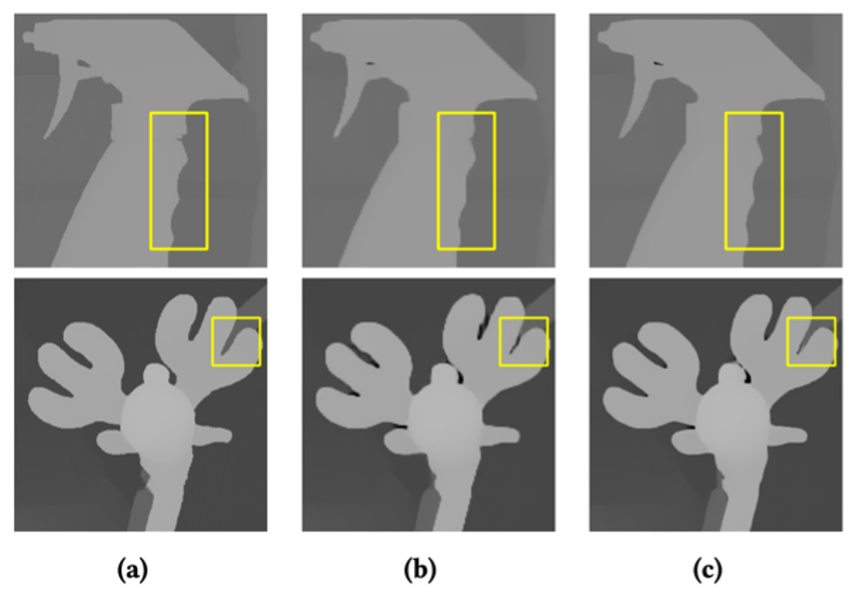
\includegraphics{figures/31.png}
	\caption{消融实验可视化结果对比}
	\label{fig:fig4-5}
	\vspace{-0.8cm}  %调整图片与下文的垂直距离
	\end{figure}

为了进一步证明高频注意力桥的有效性,本文通过将单目深度估计子网络的特征未经任何处理地馈入到深度图像超分辨率重建子网络来代替它,并在 Middlebury 数据集上进行了训练,以及在 Middlebury 2005数据集上进行了上采样因子为 $\times 8$ 的对比实验,量化指标结果如表 \ref{tab:tab4-5} 所示(w/o HABdg 指的是通过直接将单目深度估计子网络的特征传递给深度图像超分辨率重建子网络代替高频注意力桥)。与简单地将通道维度上的特征级联并送入深度图像超分辨率重建网络相比,本文提出的高频注意力桥可以提供更有效的高频指导以提高性能。

\begin{table}[]
\caption{针对高频注意力桥的消融研究量化对比}
\label{tab:tab4-5}
\setlength{\tabcolsep}{3.7mm}{
\begin{tabular}{c|cccccc|c}
\toprule[1.5pt]
          & Art  & Books & Dolls & Laundry & Mobius & Reindeer & Avg.  \\\hline
w/ HABdg  & 0.58 & 0.24  & 0.34  & 0.34    & 0.26   & 0.31     & 0.343 \\
w/o HABdg & 0.65 & 0.25  & 0.37  & 0.38    & 0.28   & 0.33     & 0.376 \\
\bottomrule[1.5pt]
\end{tabular}}
\end{table}

\section{本章小结}

本章主要介绍了本文所设计的实验及其测试结果,包括在不同数据集上与最新方法的可视化对比和评价指标的比较。首先,介绍了本文采用的公开基准数据集和评估指标,并对有关实验的详细配置进行了阐明,然后介绍了本文提出的单目深度估计和深度图像超分辨率重建联合学习网络在 Middlebury 数据集上不同上采样因子的实验结果及分析,并与最新的深度超分辨率重建算法的结果进行了对比。同样,本文也将 NYU v2 数据集上不同上采样因子的实验结果与代表性的方法进行了对比和分析。此外,本文通过设计详尽的消融实验探究了所提出网络设计的有效性,验证了两个桥接器对提升深度图像超分辨率重建任务性能的积极作用。

\chapter{结论}
\markboth{正文}{正文}

本文探索了一种联合学习框架,该框架结合了深度图像超分辨率重建和单目深度估计两个任务,可以在不添加任何其他监督信息的情况下提升深度图像超分辨率重建的性能。

高分辨率彩色图像由于其具有与深度图像的结构相似性且容易获得,被广泛用于为深度图像超分辨率重建提供先验信息。但现有颜色指导的深度图像超分辨率重建算法通过额外分支提取到的指导信息,并没有很好地面向深度模态,因此可能在两种模态结构不一致的区域造成纹理复制等问题。而单目深度估计旨在将场景从光度表示映射到几何表示,换言之,在连续的训练和学习过程中,单目深度估计实现了从彩色图像到深度图像的跨模态信息转换。因而面向单目深度估计学习到的彩色图像特征更适合指导深度图像超分辨率重建。

本文的核心思想是如何设计两个子网络(即深度图像超分辨率重建子网络和单目深度估计子网络)之间的交互,由此本文提出了两个桥接器。特征编码阶段中的高频注意力桥将从单目深度估计子网络学习到的彩色高频信息传输到深度图像超分辨率重建子网络,从而可以提供更接近深度模态的颜色指导信息。遵循简单任务指导困难任务的原则,在特征解码阶段交换了两个任务的指导角色,深度图像超分辨率重建子网络通过内容引导桥为单目深度估计子网络在深度特征空间提供内容引导。全面的实验表明,本文提出的方法达到了具有竞争力的性能,尤其是在上采样因子较大的情况下。

此外,本文提出的网络结构具有高度的可移植性,可以为关联深度图像超分辨率重建任务和单目深度估计任务提供范例。在未来的工作中,可以通过替换不同的单目深度估计子网络和深度图像超分辨率重建子网络以更进一步验证本文提出的交互模式的普适性,并在提升深度图像超分率重建性能的同时加快网络的推理速度。


%========================================================================%
% 参考文献
%========================================================================%
\newpage
\pagestyle{bjtufancy}

\nocite{*} % 显示.bib文件中的所有参考文献,无论正文是否引用

\printbibliography[heading=bjtuheading]
\addcontentsline{toc}{part}{参考文献}
\cleardoublepage
%========================================================================%
% 致谢
%========================================================================%
%\thankspage
\begin{thanks}
[鼠标左键单击选择该段落,输入替换之。内容为小四号宋或楷体字。] 放置在参考文献页后,对象包括:1)国家科学基金,资助研究工作的奖学金基金,合同单位,资助或支持的企业、组织或个人。2)协助完成研究工作和提供便利条件的组织或个人。3)在研究工作中提出建议和提供帮助的人。4)给予转载和引用权的资料、图片、文献、研究思想和设想的所有者。5)其他应感谢的组织和个人。
\end{thanks}
%========================================================================%
% 附录
%========================================================================%
\begin{appendix}

\section*{附录A\hspace{1em}程序代码【1级标题,三号黑体字】}
\zihao{5} 
附录是作为论文主体的补充项目,并不是必须的。\par
论文的附录依序用大写正体英文字母A、B、C……编序号,如:附录A。

\section*{附录B\hspace{1em}工程图纸【1级标题,三号黑体字】}

\end{appendix}

\end{document}
